%!TEX root = ../dolgozat.tex
\chapter{Megvalósítás}
\label{ch:megvalositas}

Ebben a fejezetben \mref{ch:tervezes}ben ismertetett terv megvalósítását mutatom be.
A teljes forráskódot nem másolom be a dolgozatba, az a mellékelt adathordozón megtalálható;
a fejezetben azokra a részekre koncentrálok, amelyek a megvalósítás során érdemi döntést
vagy technikai nehézséget jelentettek. A rendszer két önálló alkalmazásból áll: egy Python
nyelvű, FastAPI keretrendszerre épülő szerveroldali alkalmazásból és egy Next.js alapú
kliensoldali alkalmazásból, amelyeket egy PostgreSQL adatbázis és a programkódok futtatására
szolgáló Docker-környezet egészít ki.

\section{A szerveroldal felépítése}

A szerveroldali alkalmazás szerkezetét a felelősségi körök szerint alakítottam ki, így az
egyes rétegek egymástól jól elkülönülnek. Az \texttt{app/models} könyvtár tartalmazza az
SQLAlchemy ORM-modelleket \cite{sqlalchemy_docs}, vagyis az adatbázis-táblák Python
osztályként megfogalmazott leírását. Az \texttt{app/schemas} könyvtárban találhatók a Pydantic
sémák, amelyek a REST API-n be- és kimenő adatok szerkezetét írják le és ellenőrzik. Az
\texttt{app/api} könyvtár négy modulja (\texttt{auth}, \texttt{exams}, \texttt{attempts},
\texttt{results}) tartalmazza a végpontokat, míg az \texttt{app/services} könyvtárban kapott
helyet az üzleti logika: a pontozás (\texttt{grading.py}), a kódfuttatás (\texttt{sandbox.py})
és a valós idejű kommunikáció (\texttt{socket\_server.py}). Az \texttt{app/core} könyvtár az
adatbázis-kapcsolatot, a jelszó- és tokenkezelést, valamint az időzónák egységes kezelését
végző segédfüggvényeket foglalja magában.

A FastAPI egyik legnagyobb előnyének a függőséginjektálást (\textit{dependency injection})
tartom \cite{fastapi_docs}. Az adatbázis-munkamenetet egy \texttt{get\_db} nevű generátorfüggvény
állítja elő, amely a kérés végén automatikusan le is zárja a kapcsolatot, így egyetlen
végpontban sem kell erről külön gondoskodni. Ugyanezt a mechanizmust használtam a
jogosultságkezelésre is: a \texttt{require\_teacher} és a \texttt{require\_student} függőségek
a végpont futása előtt ellenőrzik a bejelentkezett felhasználó szerepkörét, és szükség esetén
\texttt{403 Forbidden} választ adnak. Így a jogosultsági szabályok egy helyen vannak megfogalmazva,
és a végpontok törzsében már csak a tényleges feladat logikája szerepel.

Az alkalmazás belépési pontja a \texttt{main.py}, ahol a FastAPI alkalmazást és a Socket.IO
szervert egyetlen ASGI alkalmazássá fűzöm össze. A \texttt{/socket.io} útvonalra érkező
kéréseket a Socket.IO szerver, minden mást a FastAPI kezel, így a két szolgáltatás ugyanazon a
porton, egyetlen \texttt{uvicorn} folyamatban fut. A fejlesztés során gyakran változott az
adatmodell, ezért készítettem egy egyszerű sémaszinkronizáló függvényt
(\texttt{sync\_missing\_columns}), amely induláskor a modellben már szereplő, de az adatbázisból
még hiányzó oszlopokat és egyedi megszorításokat adatvesztés nélkül pótolja. Éles rendszerben
erre a célra egy migrációs eszköz (például az Alembic) volna a megfelelő választás, a prototípus
szintjén azonban ez a megoldás elegendőnek bizonyult.

\section{Hitelesítés és jogosultságkezelés}

A felhasználók jelszavát a rendszer soha nem tárolja nyílt szövegként: regisztrációkor a
\texttt{passlib} könyvtár bcrypt algoritmussal sózott hash-t képez belőle
\cite{provos1999bcrypt}, bejelentkezéskor pedig ezzel hasonlítja össze a megadott jelszót. A
bcrypt előnye, hogy szándékosan lassú, és a munkatényezője növelhető, így a nyers erővel történő
jelszótörés költsége a hardverek fejlődésével együtt emelhető.

Sikeres bejelentkezés után a szerver egy JSON Web Tokent (JWT) állít ki \cite{rfc7519}, amely a
felhasználó e-mail címét és a lejárati időt tartalmazza, és HS256 algoritmussal, a szerver titkos
kulcsával van aláírva. A token egy napig érvényes; a kliens minden további kérésnél az
\texttt{Authorization: Bearer} fejlécben küldi vissza. A JWT előnye, hogy a szervernek nem kell
munkamenet-állapotot tárolnia: az aláírás ellenőrzésével eldönthető, hogy a token hiteles-e. A
szerepkört szándékosan nem a tokenbe írtam, hanem minden kérésnél az adatbázisból olvasom ki,
így egy szerepkör-módosítás azonnal érvényre jut.

Az oktatói regisztrációt meghívókódhoz kötöttem, hiszen ellenkező esetben bármely hallgató
oktatóként regisztrálhatna, és hozzáférhetne a vizsgák megoldókulcsaihoz. A meghívókód
ellenőrzésénél a \texttt{hmac.compare\_digest} függvényt használtam a szokásos egyenlőségvizsgálat
helyett, mert ez az összehasonlítást a bemenettől független idő alatt végzi el, így időzítéses
támadással (\textit{timing attack}) sem lehet a kódot karakterenként kitalálni.

A jogosultságkezelés másik fontos eleme a tulajdonjog ellenőrzése. Egy oktató csak a saját
maga által létrehozott vizsgát tekintheti meg, módosíthatja és értékelheti; ezt a
\texttt{get\_owned\_exam} segédfüggvény biztosítja, amelyet minden oktatói végpont meghív.
A hallgatók hasonlóképpen kizárólag a saját kitöltésükhöz férnek hozzá.

\section{A megoldókulcs védelme}

A rendszer tervezésekor az egyik legfontosabb követelmény az volt, hogy a megoldókulcs semmilyen
módon ne juthasson el a hallgatóhoz (lásd \aref{sec:kovetelmenyek}. szakaszt). Ezt a Pydantic
sémák szintjén oldottam meg: a feladatoknak két külön nézete van. A \texttt{QuestionPublic}
séma csak a feladat szövegét, pontértékét, a válaszlehetőségeket és a kódfeladatok nyilvános
példatesztjeit tartalmazza, míg az ebből származtatott \texttt{QuestionTeacher} séma ezt a
megoldókulccsal egészíti ki. Mivel a FastAPI a válasz előállításakor mindig a végponthoz rendelt
séma mezőit szerializálja, a hallgatói végpontok akkor sem adhatnák ki a megoldókulcsot, ha az
az objektumban egyébként jelen van.

Ugyanez a gondolat érvényesül a vizsga folyamata közben is. A hallgató a feladatokat csak a vizsga
elindításakor kapja meg, a vizsgalistában csak a vizsga címe, időpontja és a feladatok száma
látszik. A pontszámokat és az oktatói visszajelzéseket a szerver csak a beadás után küldi el, a
kódfeladatok rejtett teszteseteiről pedig a hallgató csak annyit tud meg, hogy sikeresek voltak-e;
a bemenetüket, az elvárt kimenetüket és az esetleges hibaüzenetet nem.

\section{A vizsgafolyamat és az időkezelés}

A vizsgafolyamat a hallgató szemszögéből három lépésből áll: elindítja a vizsgát, kitölti a
feladatokat, majd beadja a megoldását. Az indításkor a szerver létrehoz egy kitöltést
(\texttt{Attempt}), és kiszámítja annak határidejét. A vizsgának van egy időablaka (kezdési és
záró időpont), valamint egy időtartama; a hallgató rendelkezésére álló idő e kettő közül a
szigorúbb:
\begin{equation}
  t_{\text{határidő}} = \min\left(t_{\text{vizsga vége}},\ t_{\text{kezdés}} + \Delta t_{\text{időtartam}}\right).
  \label{eq:hatarido}
\end{equation}
Így ha valaki a vizsgaablak vége előtt tíz perccel kezd hozzá egy hatvanperces vizsgához, akkor
is csak tíz perce marad, ami megfelel a hagyományos vizsgák gyakorlatának.

Az adatbázisban a kitöltésekre egyedi megszorítás vonatkozik a hallgató és a vizsga azonosítójára,
vagyis minden hallgató egy vizsgát csak egyszer tölthet ki. Ez a megszorítás egy versenyhelyzetet
is kezel: ha a kliens két indítási kérést küld szinte egyszerre (például dupla kattintás miatt),
akkor a második beszúrás \texttt{IntegrityError} kivétellel meghiúsul, a szerver pedig ilyenkor
visszagörgeti a tranzakciót, és a már létrejött kitöltést adja vissza.

A határidő betartását a szerver ellenőrzi, a kliens oldali visszaszámláló csupán tájékoztató
jellegű. Minden módosító kérésnél (válasz mentése, kód futtatása) az \texttt{is\_active} függvény
megvizsgálja, hogy a kitöltés még nyitott-e. A hálózati késleltetés miatt 30 másodperces türelmi
időt hagytam, hogy az utolsó pillanatban elküldött mentés ne vesszen el. Lejárt kitöltés esetén
a szerver \texttt{409 Conflict} választ ad, és lezárja a kitöltést. A lezárást nem egy külön
időzített folyamat végzi, hanem ,,lusta'' módon történik: bármely végpont, amely a kitöltéshez
hozzáfér (a hallgatói nézet, a hallgató eredménylistája vagy az oktatói eredményoldal), először
meghívja a \texttt{finalize\_if\_expired} függvényt. Ennek az az előnye, hogy nincs szükség
háttérfolyamatra, és a lejárt kitöltések akkor is lezárulnak, ha a hallgató egyszerűen bezárta a
böngészőt.

A kliens oldalon két megoldás teszi megbízhatóvá a kitöltést. Az egyik az automatikus mentés:
a válasz minden módosítás után 800 milliszekundumos késleltetéssel (\textit{debounce}) mentődik,
így gépelés közben nem keletkezik fölösleges hálózati forgalom, a hallgató mégsem veszít el
munkát. A még el nem mentett válaszok miatt a böngésző figyelmeztet, ha a hallgató el akarja
hagyni az oldalt, beadáskor pedig a kliens először minden függőben lévő mentést elküld. A másik
megoldás az óraeltérés kezelése. A hallgató számítógépének órája eltérhet a szerverétől, ezért a
szerver minden válaszában elküldi a saját aktuális idejét, a kliens pedig ebből kiszámítja az
eltérést, és a visszaszámlálót ezzel korrigálja. Amikor a hátralévő idő elfogy, a kliens
automatikusan beadja a vizsgát.

\section{Az automatikus pontozás}
\label{sec:pontozas}

A pontozás logikáját a \texttt{grading.py} modulban, feladattípusonként külön valósítottam meg.
Az egyválasztós és az igaz--hamis feladatoknál a hallgató akkor kapja meg a teljes pontszámot, ha
a megjelölt válasza megegyezik a helyessel. A több helyes választ is tartalmazó feladatoknál a
puszta egyezés túl szigorú volna, a helyes jelölések egyszerű megszámolása viszont lehetővé tenné,
hogy valaki minden lehetőséget megjelöljön. Ezért a rendszer részpontot ad, de a hibás jelöléseket
levonja:
\begin{equation}
  P = \max\!\left(0,\ \frac{|S \cap H| - |S \setminus H|}{|H|}\right) \cdot P_{\max},
  \label{eq:tobbvalasz}
\end{equation}
ahol $S$ a megjelölt, $H$ a helyes válaszok halmaza, $P_{\max}$ pedig a feladat pontértéke. Ha
például három helyes válaszból a hallgató kettőt és egy hibásat jelöl meg, akkor a pontszám
$(2-1)/3$, vagyis a maximális pontszám egyharmada. A nullánál húzott alsó korlát miatt egy feladat
negatív pontot nem eredményezhet.

A rövid szöveges válaszoknál az oktató több elfogadott választ is megadhat. Az összehasonlítás előtt
a rendszer mindkét oldalt normalizálja: kisbetűssé alakítja (a Unicode szerinti
\texttt{casefold} művelettel, amely az ékezetes betűket is helyesen kezeli), és a többszörös
szóközöket egyetlen szóközre cseréli. Ha mindkét érték számként értelmezhető, akkor a rendszer a
számértékeket hasonlítja össze, így a magyar és az angol tizedesjelölés (\texttt{3,14} és
\texttt{3.14}) egyaránt elfogadott. A kifejtős feladatok értelemszerűen nem pontozhatók
automatikusan; ezek beadás után ,,javításra vár'' állapotba kerülnek, és az oktató értékeli őket.

A kézi értékelés minden feladattípusnál elérhető: az oktató felülírhatja az automatikus pontszámot,
és szöveges visszajelzést fűzhet a válaszhoz. Az adatmodellben ezért külön mező tárolja az
automatikus és a kézi pontszámot; ha kézi pontszám létezik, az az érvényes. Ennek köszönhetően a
felülírás visszavonható, és utólag is látszik, mit számolt a rendszer.

\section{Biztonságos kódfuttatás Docker-sandboxban}
\label{sec:sandbox}

A programozási feladatok értékelése a rendszer legérzékenyebb része, hiszen a szerver ilyenkor
egy ismeretlen személy által írt, tetszőleges programkódot futtat. Egy rosszindulatú (vagy
egyszerűen hibás) program megpróbálhat fájlokat olvasni a szerverről, hálózati kapcsolatot
nyitni, elfogyasztani a memóriát, vagy végtelen számú folyamatot indítani. Ezért a kódot
Docker-konténerben futtatom \cite{merkel2014docker}, amelyre szigorú korlátozásokat alkalmazok.
Ezeket \aref{tab:sandbox}. táblázat foglalja össze, a konténer indítási paramétereit pedig
\aref{py:sandbox}. programkód mutatja.

\begin{table}[H]
  \centering
  \caption{A sandbox konténer korlátozásai}
  \label{tab:sandbox}
  \begin{tabularx}{\textwidth}{@{}lX@{}}
    \toprule
    Korlátozás & Érték, cél \\
    \midrule
    Hálózat             & nincs -- adatszivárgás és külső támadás ellen \\
    Memória             & 128 MB \\
    CPU                 & 0,5 mag \\
    Folyamatok száma    & legfeljebb 64 (\enquote{fork bomb} ellen) \\
    Fájlrendszer        & csak olvasható; \texttt{/tmp}: 16 MB-os tmpfs \\
    Jogosultságok       & minden capability eldobva, \texttt{no-new-privileges}; a kód \texttt{nobody}-ként fut \\
    Időkorlát           & 5 mp tesztesetenként \\
    Kimenet             & legfeljebb 64 KB tesztesetenként \\
    \bottomrule
  \end{tabularx}
\end{table}

\begin{python}[caption={A sandbox konténer indítási paraméterei (\texttt{sandbox.py}, részlet)},label=py:sandbox]
run_kwargs = dict(
    image=SANDBOX_IMAGE,
    command=["python", "-c", _RUNNER],
    network_mode="none",
    mem_limit="128m",
    nano_cpus=500_000_000,
    pids_limit=64,
    read_only=True,
    tmpfs={"/tmp": "size=16m,mode=1777"},
    cap_drop=["ALL"],
    cap_add=["SETUID", "SETGID", "KILL"],
    security_opt=["no-new-privileges"],
)
\end{python}

Az első változatban minden tesztesethez külön konténert indítottam, ez azonban egy tíz tesztesetből
álló feladatnál már több másodperces várakozást jelentett, mivel a konténer indítása önmagában is
időigényes. Ezért a végleges megoldásban egy kiértékeléshez egyetlen konténer indul, amelyben egy
rövid vezérlőprogram (\textit{runner}) egymás után futtatja le a hallgató kódját az összes
tesztbemenettel, majd az eredményeket JSON formátumban adja vissza. A konténer indításának
költsége így csak egyszer jelentkezik.

Ez a megoldás azonban felvet egy újabb biztonsági kérdést: ha a hallgató kódja ugyanabban a
környezetben fut, mint a vezérlőprogram, akkor elvileg meghamisíthatná az eredményeket. Ezt úgy
zártam ki, hogy a vezérlőprogram rendszergazdai jogokkal fut, a hallgató kódját viszont egy
alfolyamatban, a jogosultságokkal nem rendelkező \texttt{nobody} felhasználóként (65534-es
azonosító) indítja el. A hallgató programjának szabványos kimenetét a vezérlőprogram csövön
(\textit{pipe}) keresztül olvassa be, így az nem keveredhet a vezérlőprogram saját kimenetével.
Ehhez kellett a \texttt{SETUID} és \texttt{SETGID} képességeket meghagyni a konténerben, a
\texttt{KILL} képességre pedig azért volt szükség, hogy az időtúllépés esetén a vezérlőprogram a
hallgató folyamatát -- az általa esetleg indított gyermekfolyamatokkal együtt -- le tudja állítani.
A \texttt{no-new-privileges} beállítás biztosítja, hogy a hallgató kódja semmilyen módon ne
szerezhessen vissza magasabb jogosultságot.

A kimenet olvasását külön szálak végzik, amelyek a megadott korlát (64 KB) fölötti részt eldobják.
Erre azért van szükség, mert egy végtelen ciklusban kiíró program néhány másodperc alatt is
gigabájtos kimenetet képes előállítani, ami a szerver memóriáját terhelné. A hallgató kódját és a
tesztbemeneteket környezeti változókban adom át a konténernek, nem pedig csatolt könyvtárban
(\textit{volume}). Ezt a döntést gyakorlati tapasztalat indokolta: Windows és Docker Desktop alatt
a könyvtárcsatolás lassú és megbízhatatlan volt, a környezeti változós átadás viszont minden
platformon egyformán működik.

A tesztek kiértékelésekor a rendszer a program kimenetét a sor eleji és végi szóközök levágása
után hasonlítja össze az elvárt kimenettel, és csak akkor tekinti a tesztet sikeresnek, ha a
program hiba nélkül (nulla kilépési kóddal) és időkorláton belül futott le. A pontszám a sikeres
tesztek arányával arányos. Fontos szempont volt az is, hogy rendszerhiba (például ha a Docker
szolgáltatás éppen nem fut) esetén a hallgató ne kapjon nulla pontot: ilyenkor a válasz
,,nem értékelt'' állapotban marad, az oktató pedig a hiba elhárítása után egyetlen gombnyomással
újraértékelheti a vizsga összes ilyen válaszát.

A hallgató a vizsga közben kétféleképpen futtathatja a kódját. A próbafuttatás saját bemenettel
vagy a nyilvános példatesztekkel fut le, és nem befolyásolja a pontszámot; ez a fejlesztői
környezetekben megszokott ,,futtatás'' gombnak felel meg. A beküldés ezzel szemben az összes, a
rejtett teszteseteket is tartalmazó tesztkészlettel értékeli a megoldást, és elmenti az eredményt.

\section{Valós idejű felügyelet}

A felügyeleti funkció célja, hogy az oktató a vizsga ideje alatt azonnal értesüljön, ha egy hallgató
elhagyja a vizsgaablakot, például egy másik böngészőfülre vált vagy másik alkalmazást nyit meg. A
kliens oldalon ezt a \texttt{useProctoring} nevű React hook valósítja meg, amely a böngésző két
eseményére iratkozik fel: az ablak fókuszvesztésére (\texttt{blur}) és a lap láthatóságának
megváltozására (\texttt{visibilitychange}). Fülváltáskor a böngésző mindkét eseményt kiváltja,
ezért egy egyszerű jelzővel biztosítottam, hogy egy elhagyás csak egyszer számítson; a jelző az
ablak visszakapott fókuszakor áll vissza (\aref{ts:proctoring}. programkód).

\begin{typescript}[caption={Az ablakelhagyás érzékelése (\texttt{useProctoring.ts}, részlet)},label=ts:proctoring]
let away = false;
const handleBlur = () => {
  if (away) return;
  away = true;
  report('WINDOW_BLUR (ablakfókusz elvesztve)');
};
const handleFocus = () => { away = false; };
const handleVisibility = () => {
  if (document.visibilityState === 'hidden' && !away) {
    away = true;
    report('TAB_HIDDEN (lapváltás / kis méret)');
  }
};
\end{typescript}

A kommunikációhoz a Socket.IO könyvtárat használtam \cite{socketio_docs}, amely WebSocket
kapcsolatot épít ki \cite{rfc6455}, de annak elérhetetlensége esetén más átviteli módra is képes
visszaváltani, és beépítetten támogatja az újracsatlakozást és a szobákat (\textit{rooms}).
Minden vizsgához tartozik egy szoba, ebbe lépnek be a vizsgázó hallgatók és a vizsgát felügyelő
oktató. Csatlakozáskor a kliens elküldi a JWT tokenjét, amelyet a szerver ugyanúgy ellenőriz, mint
a REST API esetén; érvénytelen tokennel a kapcsolat létre sem jön. A felhasználó nevét és
szerepkörét a szerver az adatbázisból olvassa ki, nem a klienstől fogadja el, így a hallgató nem
adhatja ki magát oktatónak. A szobába lépésnél a szerver további ellenőrzést végez: oktató csak a
saját vizsgája szobájába léphet be, hallgató pedig csak akkor, ha az adott vizsgán folyamatban lévő
kitöltése van.

Amikor a hallgató kliense szabálysértést jelez, a szerver megnöveli a kitöltéshez tartozó
számlálót az adatbázisban, majd továbbítja az eseményt a szoba többi résztvevőjének, vagyis az
oktatónak. Azért döntöttem az adatbázisban való tárolás mellett, mert így a számláló nem vész el,
ha a hallgató frissíti az oldalt, vagy ha az oktató később csatlakozik: belépéskor az oktató
pillanatképet (\textit{snapshot}) kap a vizsga összes kitöltésének aktuális állapotáról, és a
szabálysértések száma az eredménylistában és a CSV exportban is megjelenik. Mivel a Socket.IO
szerver aszinkron módon működik, az SQLAlchemy szinkron adatbázis-műveletei viszont blokkolnák az
eseményhurkot, ezeket az \texttt{asyncio.to\_thread} függvénnyel külön szálon futtatom. A szerver
azt is nyilvántartja, hogy egy hallgató hány böngészőfülön csatlakozik, így az oktató csak akkor
látja ,,offline'' állapotúnak, ha az összes kapcsolata megszakadt.

Fontosnak tartom kiemelni, hogy ez a megoldás nem nyújt teljes védelmet a csalás ellen: egy
második eszközt (például mobiltelefont) használó hallgatót a böngésző nem képes érzékelni. A
funkció célja inkább a visszatartás és az oktató tájékoztatása; a webkamerás vagy
mesterséges intelligenciára épülő felügyelet \mref{ch:koncepcio}ben bemutatott adatvédelmi és
etikai kérdések miatt nem volt célja ennek a dolgozatnak.

\section{A felhasználói felület}
\label{sec:felulet}

A kliensoldali alkalmazást a Next.js keretrendszer App Router megoldásával készítettem
\cite{nextjs_docs}, a megjelenéshez a Tailwind CSS segédosztályait használtam. Az oldalak a
szerepkörök szerint két csoportra oszlanak. A hallgatói műszerfalon a hallgató látja az elérhető
vizsgákat és a korábbi eredményeit. A vizsgaoldal rögzített fejlécében a hátralévő idő, a
felügyeleti kapcsolat állapota és az ablakváltások száma látható, a feladatok között pedig egy
gombsorban navigálhat, ahol pipa jelzi, mely feladatokra válaszolt már; az éppen szerkesztett
feladatnál az automatikus mentés állapota (,,Mentés\ldots'', ,,Mentve'') is megjelenik. Az oktatói felületen a vizsgák kezelése mellett egy vizsgához három fül tartozik: a
feladatszerkesztő, az élő monitor és az eredmények.

A feladatszerkesztő típusonként eltérő űrlapot jelenít meg: választós feladatnál a
válaszlehetőségek és a helyes válaszok megjelölése, rövid válasznál az elfogadott válaszok,
kódfeladatnál pedig a tesztesetek szerkesztése jelenik meg, ahol minden tesztesetről megadható,
hogy nyilvános példateszt vagy rejtett teszt legyen. Az űrlapon megadott adatokat a szerver a
Pydantic sémákban megfogalmazott szabályok szerint is ellenőrzi és egységes formára hozza, így
hibás megoldókulcs (például nem létező válaszlehetőségre mutató index) nem kerülhet az
adatbázisba.

Az eredmények fülön az oktató hallgatónként áttekintheti a válaszokat, pontozhatja a kifejtős
feladatokat, és az eredményeket CSV fájlba exportálhatja. Az export kialakításánál a magyar
nyelvű Excel sajátosságaihoz igazodtam: pontosvesszőt használtam elválasztóként, és a fájl elejére
UTF-8 bájtsorrend-jelzőt (BOM) írtam, mert enélkül az Excel hibásan jeleníti meg az ékezetes
karaktereket.

A programkód szerkesztésére egy egyszerű, egyenközű betűtípussal megjelenített szövegmezőt
használtam. Egy fejlettebb, szintaxiskiemelést nyújtó szerkesztő (például a Monaco Editor)
beépítése kényelmesebbé tenné a munkát, ezt a továbbfejlesztési lehetőségek között tartom számon.

A hallgatói vizsgaoldalt programozási feladat közben \aref{fig:vizsgaoldal_kod}. ábra mutatja. A
fejlécben a visszaszámláló, a felügyelet állapota és az ablakváltások száma látható, alatta a
feladatok gombsora. A feladat szövege alatt a nyilvános példatesztek jelennek meg, a bal oldali
szerkesztőben a hallgató a kódját írja, a jobb oldali konzolban pedig a próbafuttatás és az utolsó
beküldés értékelésének eredménye látható.

\begin{figure}[H]
  \centering
  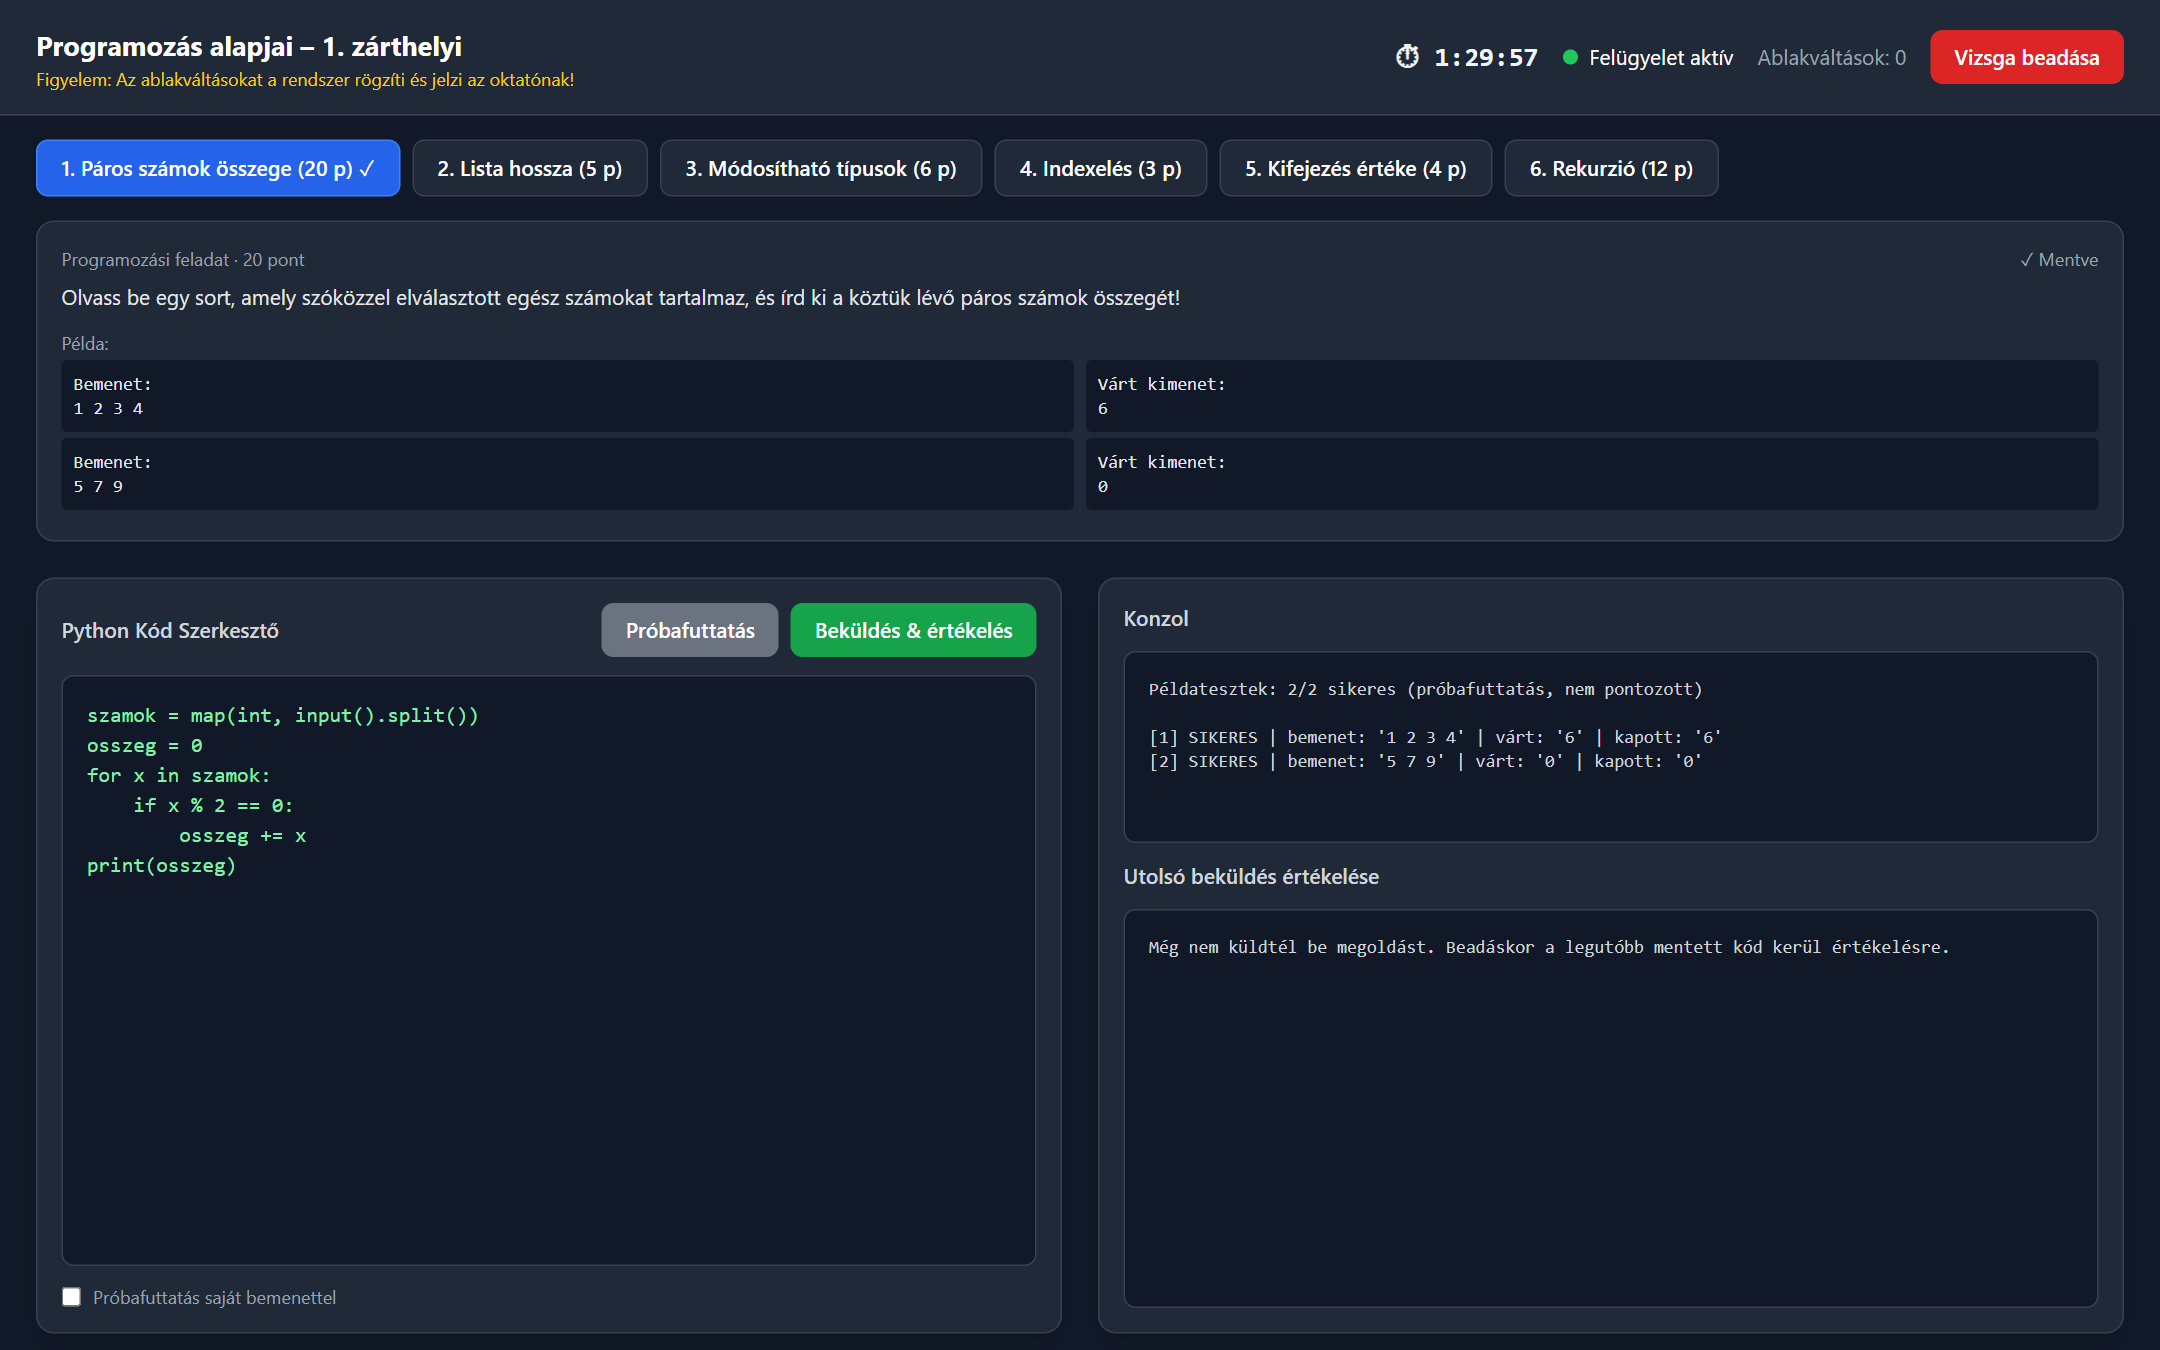
\includegraphics[width=\textwidth]{images/vizsgaoldal_kod.png}
  \caption{A hallgatói vizsgaoldal programozási feladattal, sikeres próbafuttatás után}
  \label{fig:vizsgaoldal_kod}
\end{figure}

Az oktatói feladatszerkesztőt \aref{fig:feladatszerkeszto}. ábra mutatja. A bal oldalon a vizsga
már felvett feladatai láthatók a megoldókulccsal együtt (a helyes válaszokat pipa jelöli), a jobb
oldali űrlap pedig a kiválasztott típushoz igazodik; az ábrán egy programozási feladat
tesztesetének megadása látható, a ,,nyilvános'' jelölővel.

\begin{figure}[H]
  \centering
  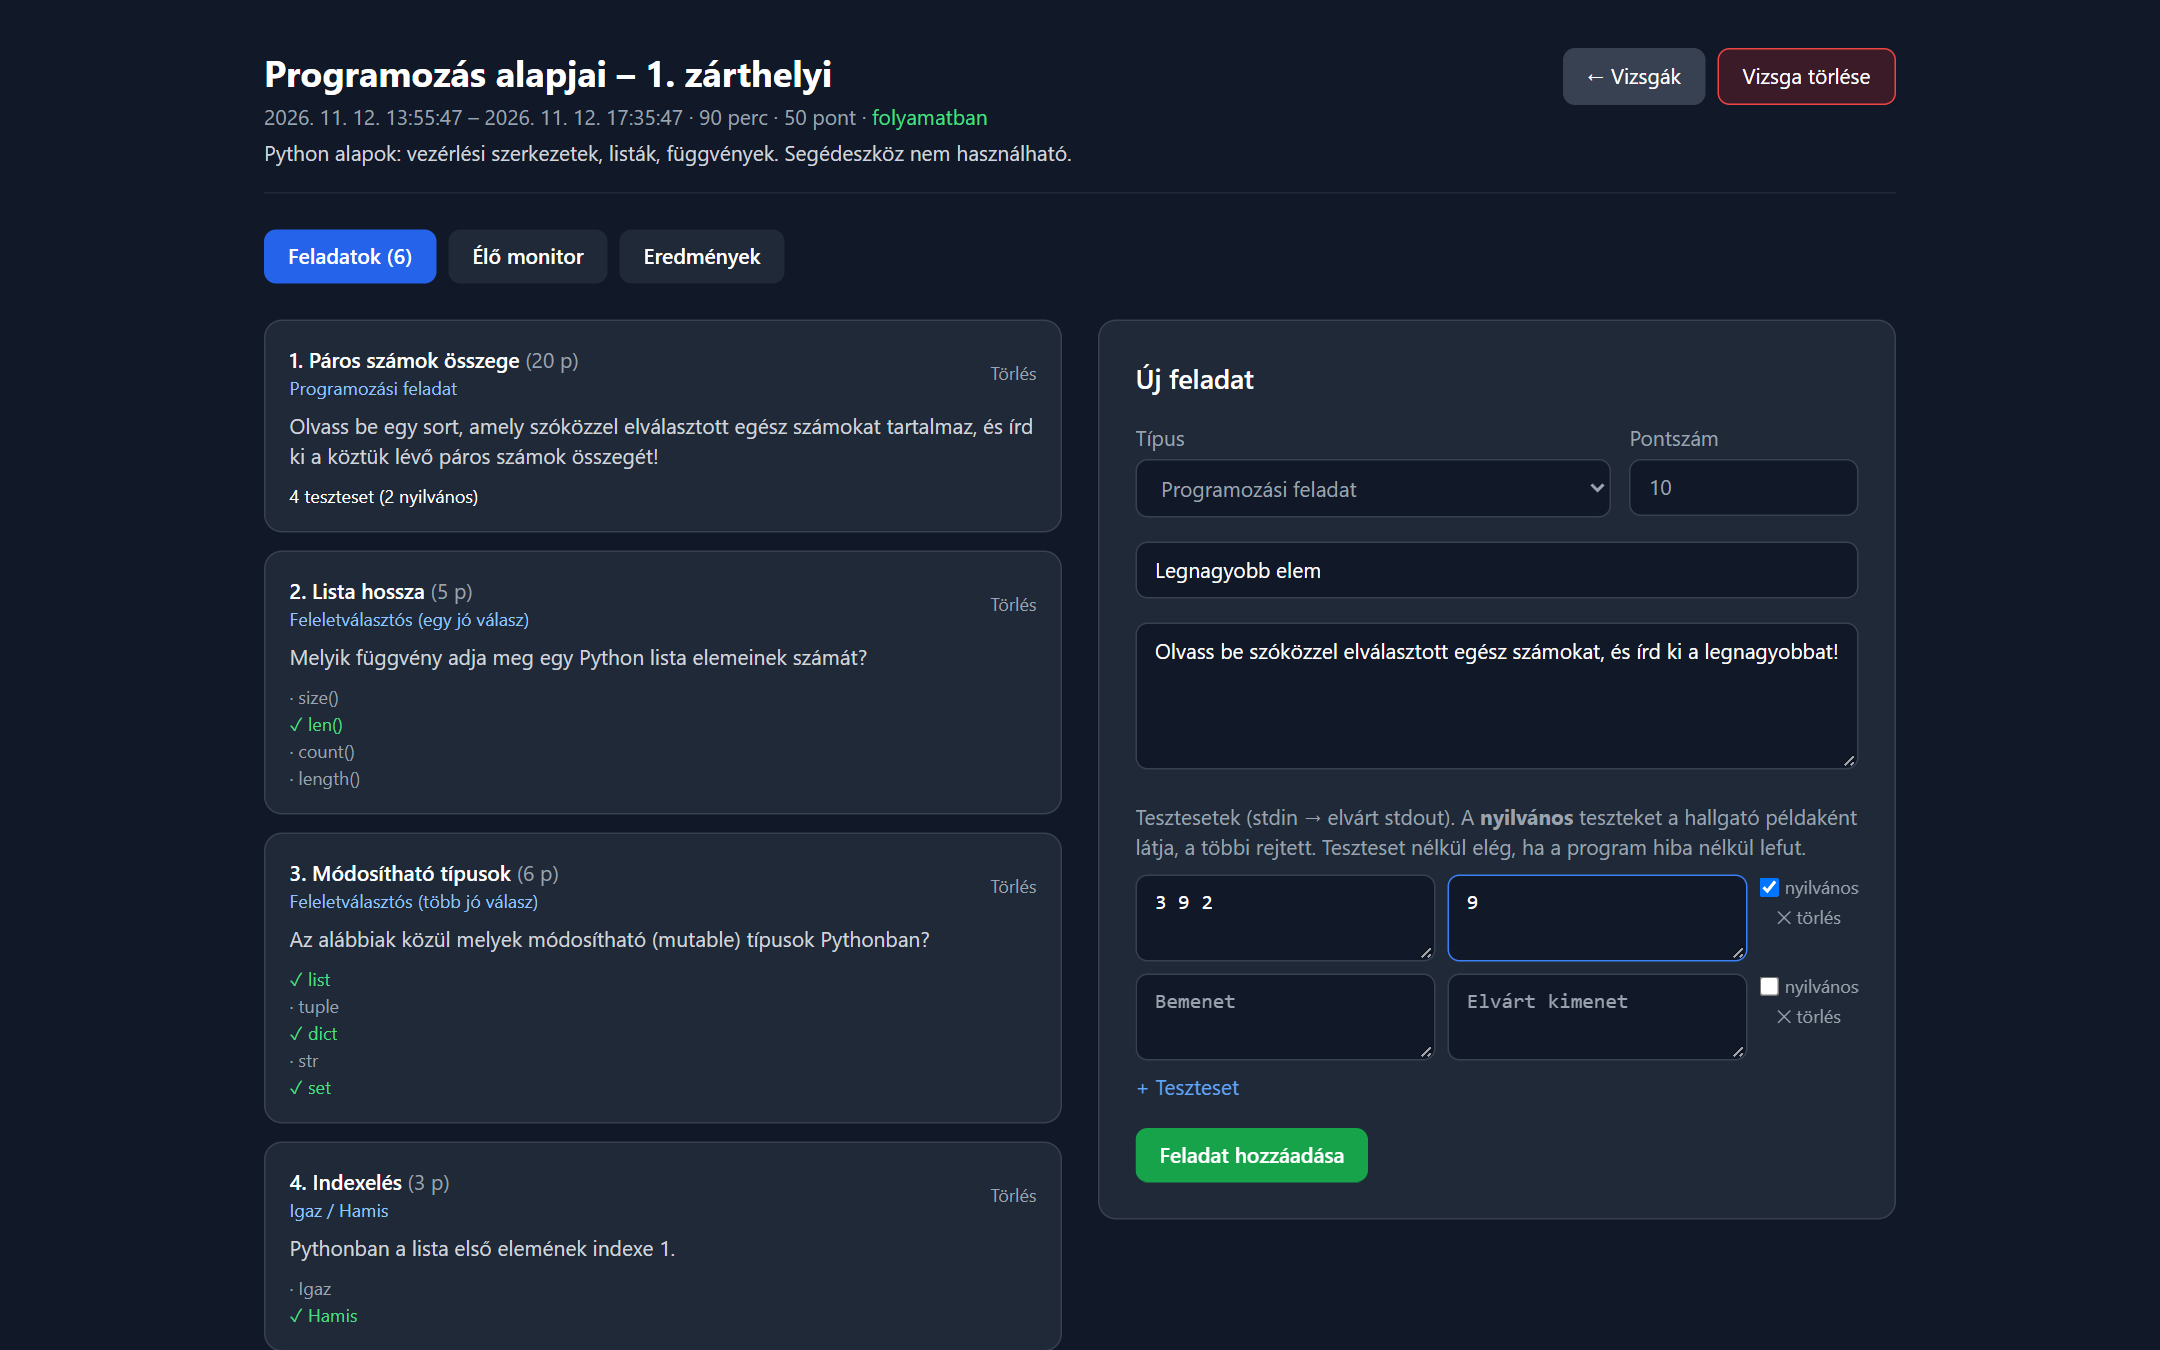
\includegraphics[width=\textwidth]{images/feladatszerkeszto.png}
  \caption{Az oktatói feladatszerkesztő programozási feladat felvétele közben}
  \label{fig:feladatszerkeszto}
\end{figure}

Az élő monitor (\mref{fig:elo_monitor}) a vizsgázókat kártyákon jeleníti meg. A kártya jelzi, hogy
a hallgató éppen dolgozik vagy már beadta a dolgozatát, valamint a figyelmeztetések számát, az
utolsó esemény típusát és időpontját. Ha egy hallgatóhoz legalább egy figyelmeztetés tartozik,
a kártyája piros keretet kap, így az oktató első ránézésre látja, kire kell figyelnie.

\begin{figure}[H]
  \centering
  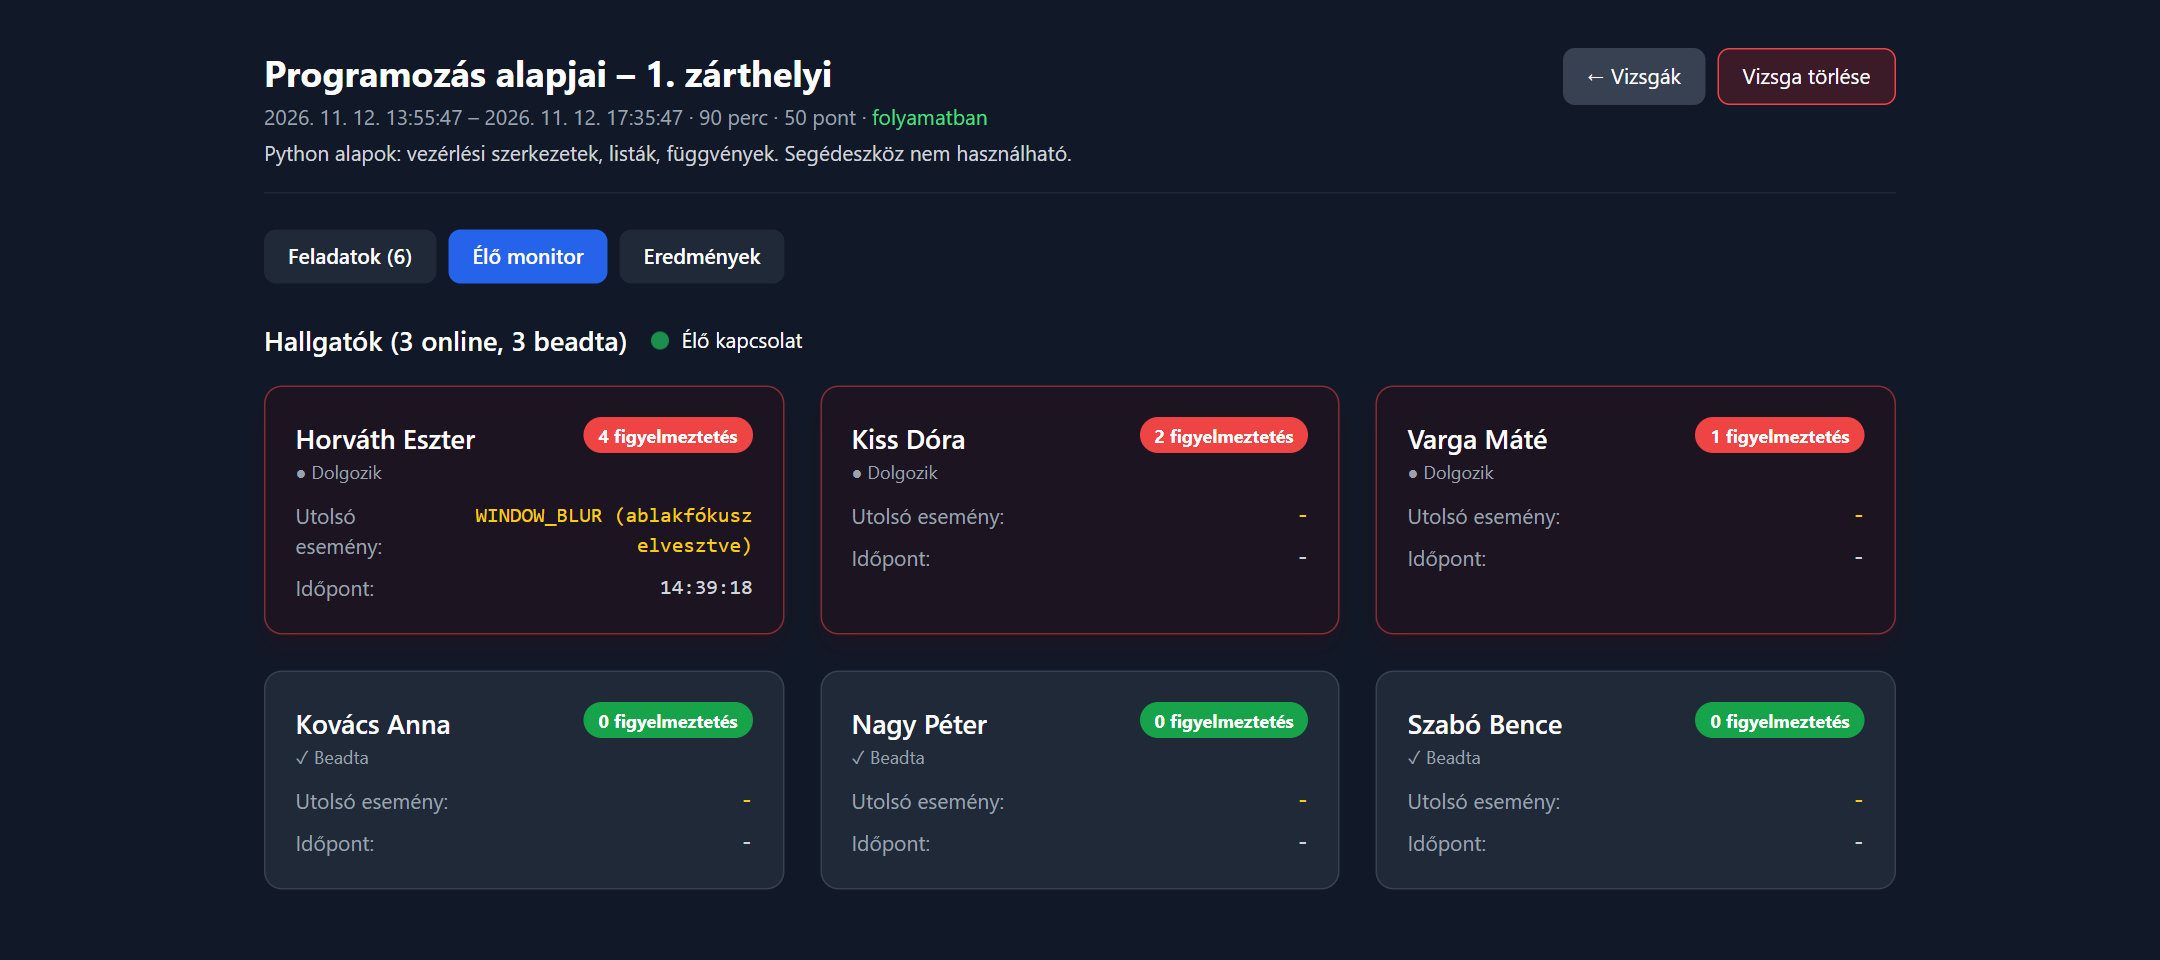
\includegraphics[width=\textwidth]{images/elo_monitor.png}
  \caption{Az élő monitor egy folyamatban lévő vizsga alatt}
  \label{fig:elo_monitor}
\end{figure}

Az eredmények fülön egy hallgató sorát lenyitva feladatonként láthatók a válaszok
(\mref{fig:eredmenyek_reszletes}). Programozási feladatnál a beküldött kód alatt a kódértékelés
részletei is megtekinthetők: az ábrán a hallgató programja a négy tesztesetből hármat teljesített,
ezért 15 pontot kapott a 20-ból. A pontszám alatti mezőkben az oktató felülírhatja az automatikus
pontot, és szöveges visszajelzést írhat.

\begin{figure}[H]
  \centering
  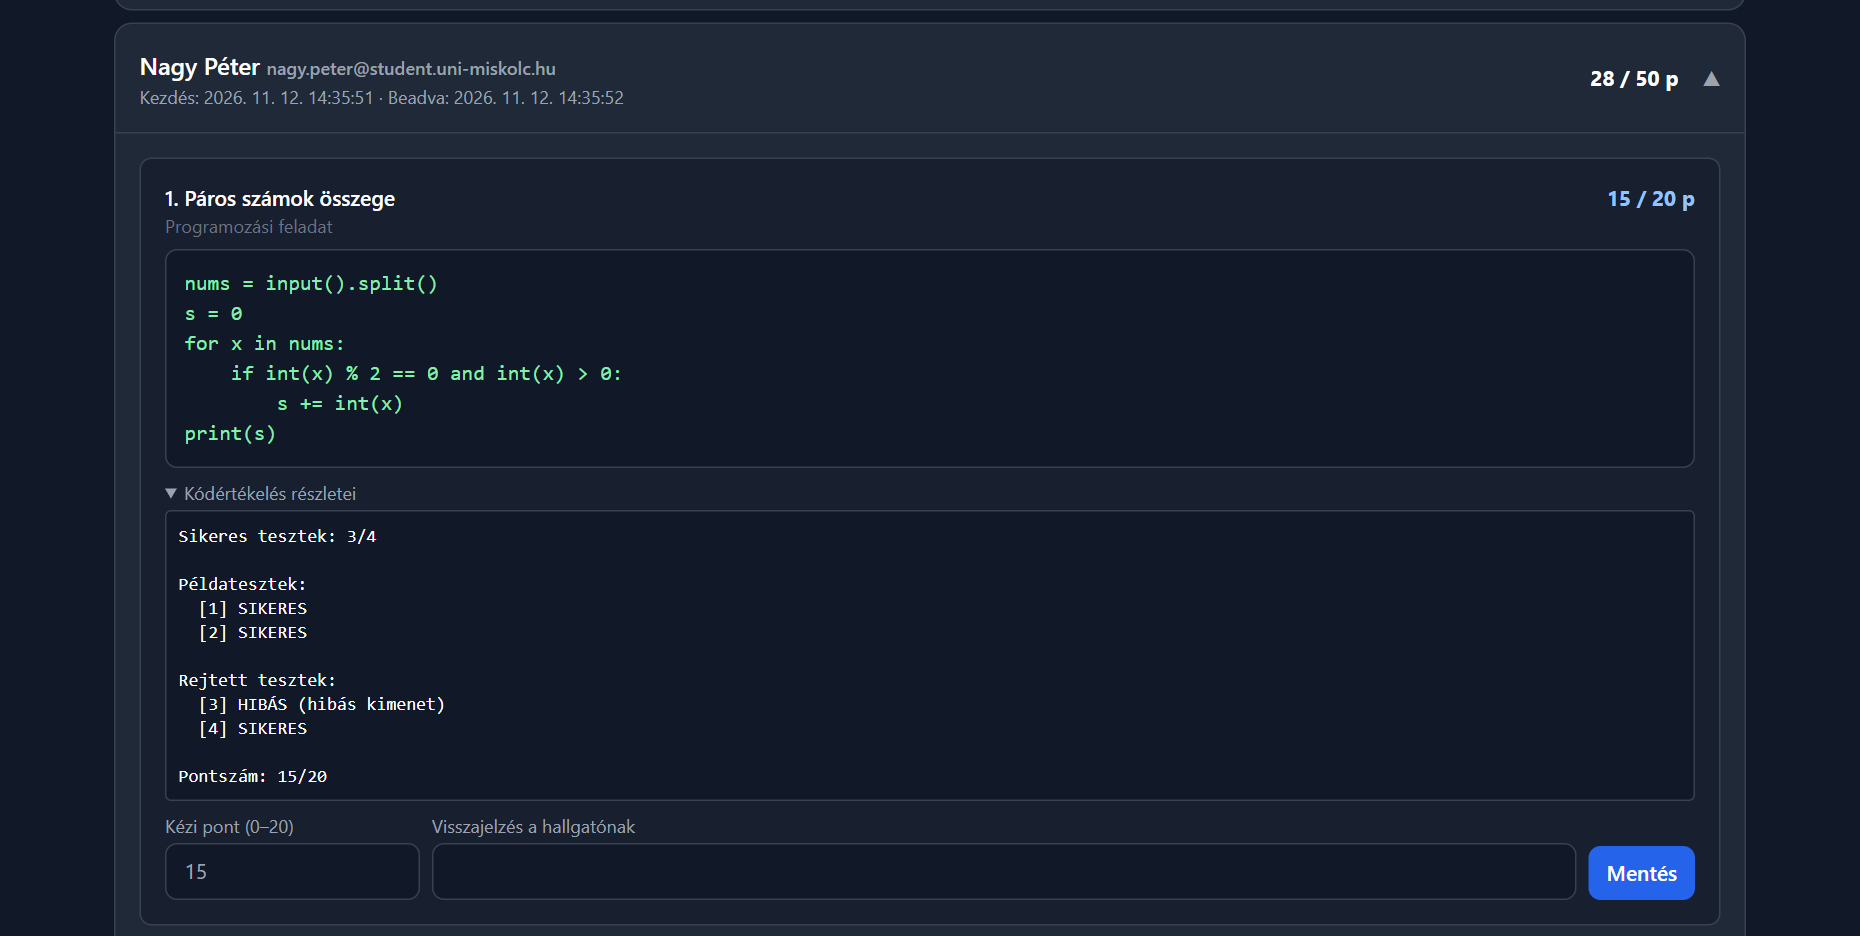
\includegraphics[width=\textwidth]{images/eredmenyek_reszletes.png}
  \caption{Egy hallgató programozási feladatra adott válasza az eredmények fülön}
  \label{fig:eredmenyek_reszletes}
\end{figure}
